\chapter{System Overview}
This chapter provides a high level overview of the hexapod, starting with the hardware, then the software, and finally the simulation
environment.
\section{Hardware}
The physical hexapod is primarily the same hexapod described in \cite{erasmus2023guidance}. For computation a JetsonNano and Teensy2.0
\ac{mcu} is used. Locomotion of the six, three degrees of freedom, legs is handled by 24 Dynamixel RX-64 servos. Sensing is handled by
a Realsense D435i \ac{rgbd} camera, which includes a \ac{imu}, although the \ac{imu} is not utilised in this system. Two marvelmind
beacons are also present on the robot, although these are not used either.

The only alterations made from the version describe in \cite{erasmus2023guidance} is the thickening of the wires powering the JetsonNano,
to prevent a voltage drop, and the replacement of 3D printed legs with laser cut aluminium legs, to prevent leg flexure.
Figure \ref{fig:hexapod} shows the hexapod in its current state.
\begin{figure}[h]
    \centering
    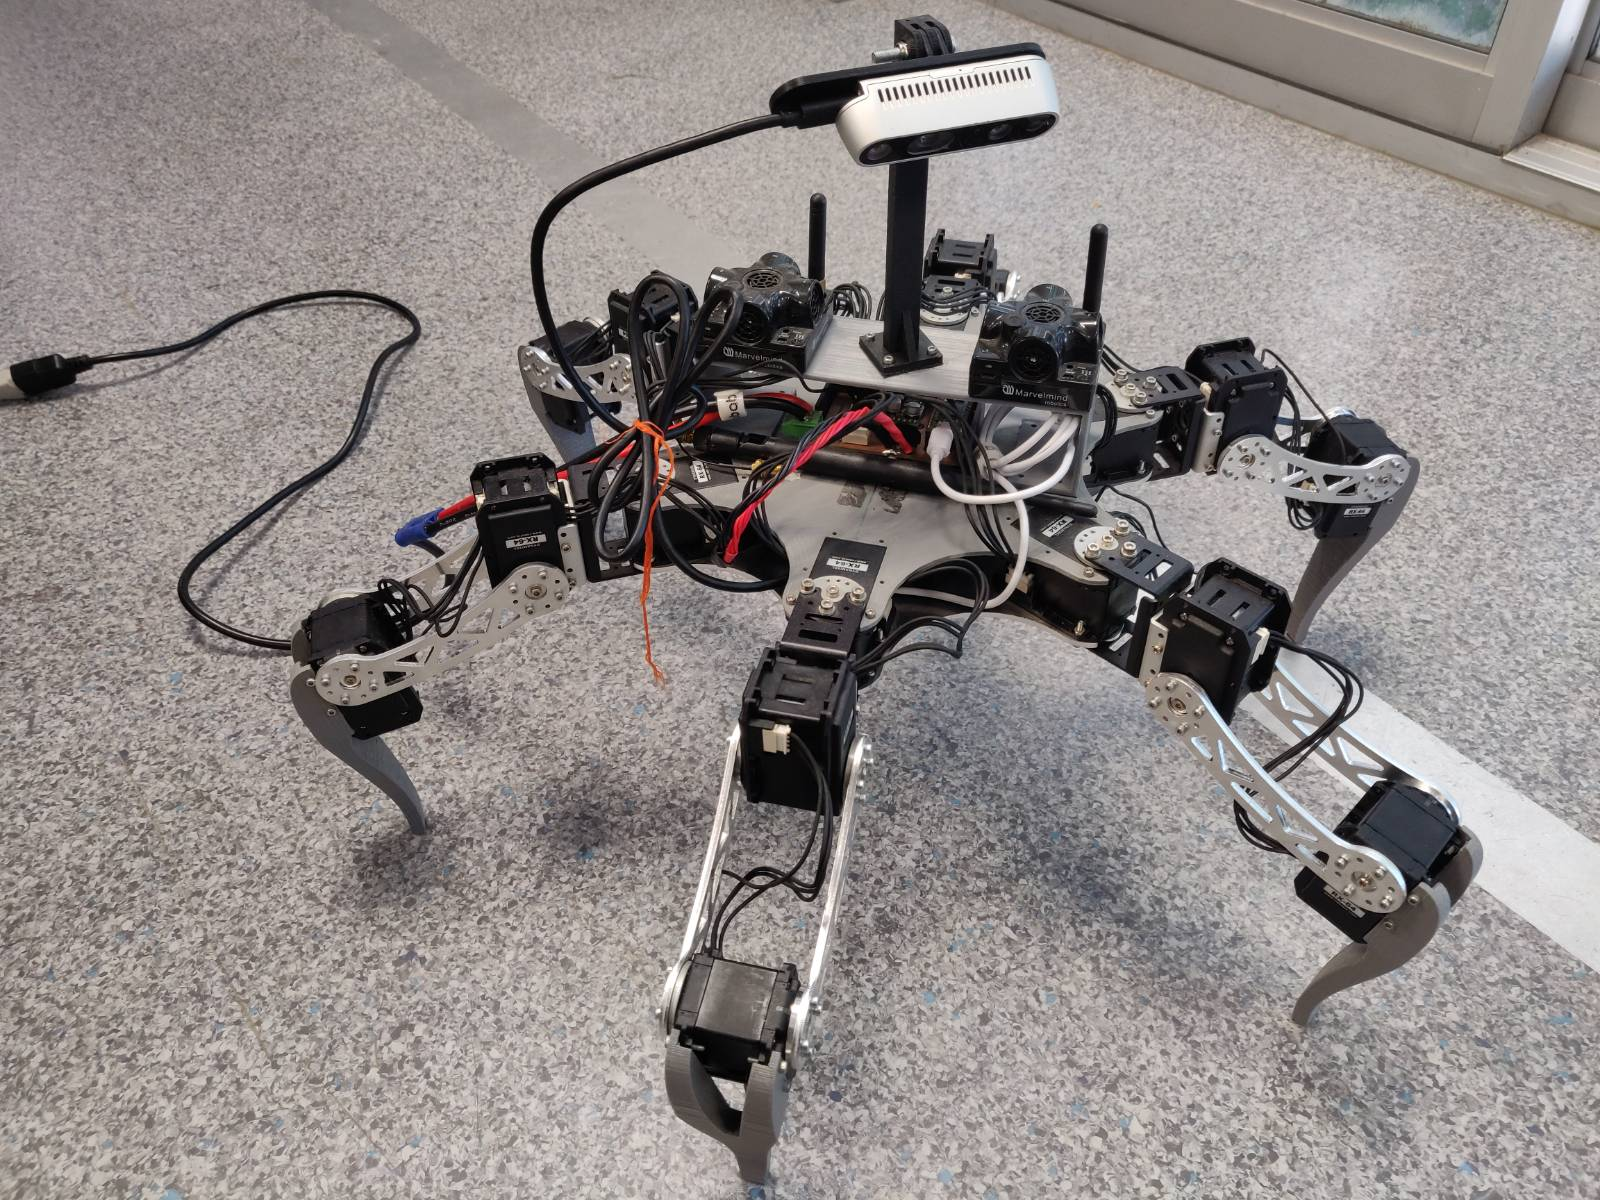
\includegraphics[height=4.9cm]{hexapod.png}
    \caption{Physical Hexapod}
    \label{fig:hexapod}
\end{figure}

\noindent
Note the power cable running off image, all tests were conducted using 14.8V
a bench power supply plugged into the batter port. This was done for convenience and can easily be swapped for a battery.

\section{Software}
The most basic software flow for a robot walking over flat terrain is shown in figure \ref{fig:basic_sys}. This system does not sense
its environment in any way and simply moves its feet in predetermined paths.
\begin{figure}[h]
    \centering
    % \hspace{-1.38cm}
    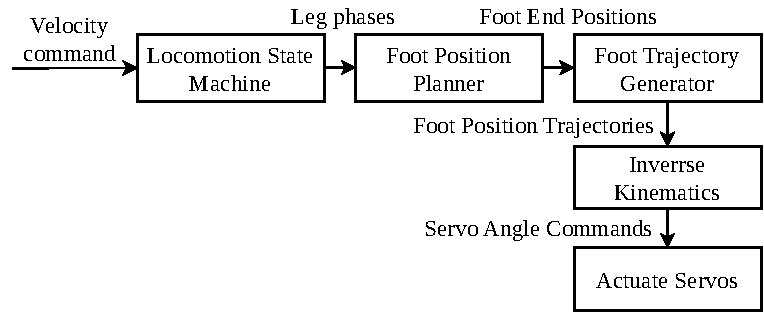
\includegraphics{Diagrams-SysDiffBlockBefore.drawio.pdf}
    \caption{Basic system operation}
    \label{fig:basic_sys}
\end{figure}

\noindent
This basic system will work well enough for walking over flat terrain, but will struggle once any
deviation in terrain height is present. Thus, the proposed, more advanced system, operates with the flow shown in figure \ref{fig:adv_sys}.
\begin{figure}[h]
    \centering
    % \hspace{-1.38cm}
    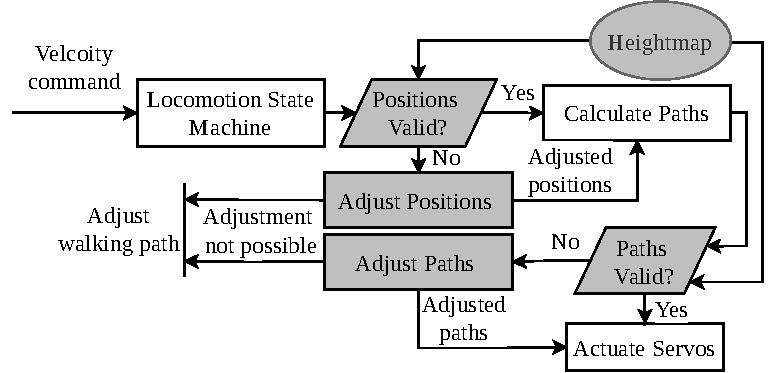
\includegraphics{Diagrams-SysDiffBlockAfter.drawio.pdf}
    \caption{Advanced system operation}
    \label{fig:adv_sys}
\end{figure}

\noindent
The advanced system uses similar components from the basic system, with some differences discussed in
later chapters, but additionally incorporates checks against a heightmap and a score map to validate, and if necessary, adjust the nominal foot 
end positions and paths to move the feet to said positions. If the nominal positions are invalid and no valid adjustment can be made the 
robot will have to change its overall path, however this is not applicable in this paper.

The goal of maneuvering rough terrain is achieved by a combination of 4 primary systems, namely, a mapping, 
foot placement optimisation, motion controller and a \ac*{slam} system. A high level overview of the system implementation can be seen
in figure \ref{fig:system_diagram}.
\begin{figure}[h]
    \centering
    % \hspace{-1.38cm}
    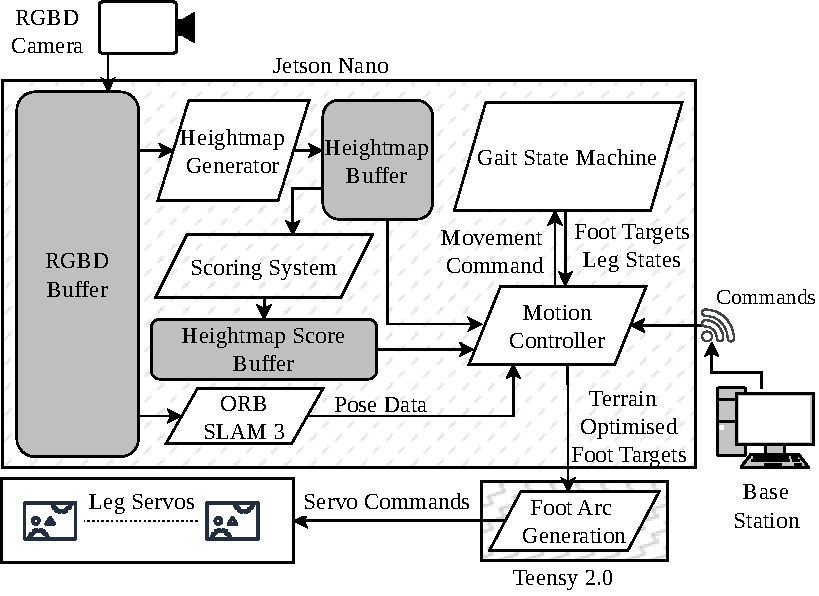
\includegraphics{HexapodSystemDiagram.drawio.pdf}
    \caption{Physical system diagram}
    \label{fig:system_diagram}
\end{figure}

The mapping system utilises the \ac*{rgbd} camera to construct a dense heightmap of the immediate surroundings of the robot, as the robot moves around old data is erased to make
way for new data. The size and resolution of the heightmap is adjustable to the available memory and computational power. The heightmap system is further covered in chapter \ref{chap:mapping}.

The foot placement optimisation system takes the heightmap as input and produces another map of equal size to the heightmap, this new map is the score map and is found by assigning a score to each
cell of the heightmap. The score is dependant on how stable of a place the cell would be for the robot to place its feet. The score map can then be used to evaluate, and adjust if necessary, the
initial foot placement proposed by the motion system. The foot placement optimisation system is further covered in chapter \ref{chap:optimisation}.

All the movement of the robot is handled by the motion system, it is comprised of a gait state machine, a foot target proposal system, a foot arc generator, and \ac{ik}.
The gait state machine selects the swinging and supporting legs during for each step, to achieve a tripod gait. The target proposal system proposes an initial target for all the feet based
on the current step parameters. Simple linear motion is not acceptable for the swinging feet, thus the foot arc generator produces a movement vector based on the remaining distance to a foots destination,
which if followed, results in a arc like motion to the destination. Finally to execute any movements, positions must be converted to angles, and velocity must be converted to
angular rate, thus, and \ac{ik} component is required. The motion system is further covered in chapter \ref{chap:motion}.

\section{Simulation}
As said in section \ref{sec:sim_research}, various simulation environments were considered, but finally \ac{mujoco} was chosen due to its excellent contact physics
simulation. The simulation includes the 24 servos, simulated as high gain, high damped angle controlled motors, similarly the \ac{rgbd} camera is also simulated.
A SLAM system does not run in the simulation, rather a amount of noise, based on \cite{macario2022comprehensive}, is added to the position directly taken from the simulation.

The software running on the simulation is largely equivalent to that running on the physical system, with only slight modification to integrate with the simulation
instead of the hardware.
Figure \ref{fig:mujoco} shows the simulation environment
\begin{figure}[h]
    \centering
    % \hspace{-1.38cm}
    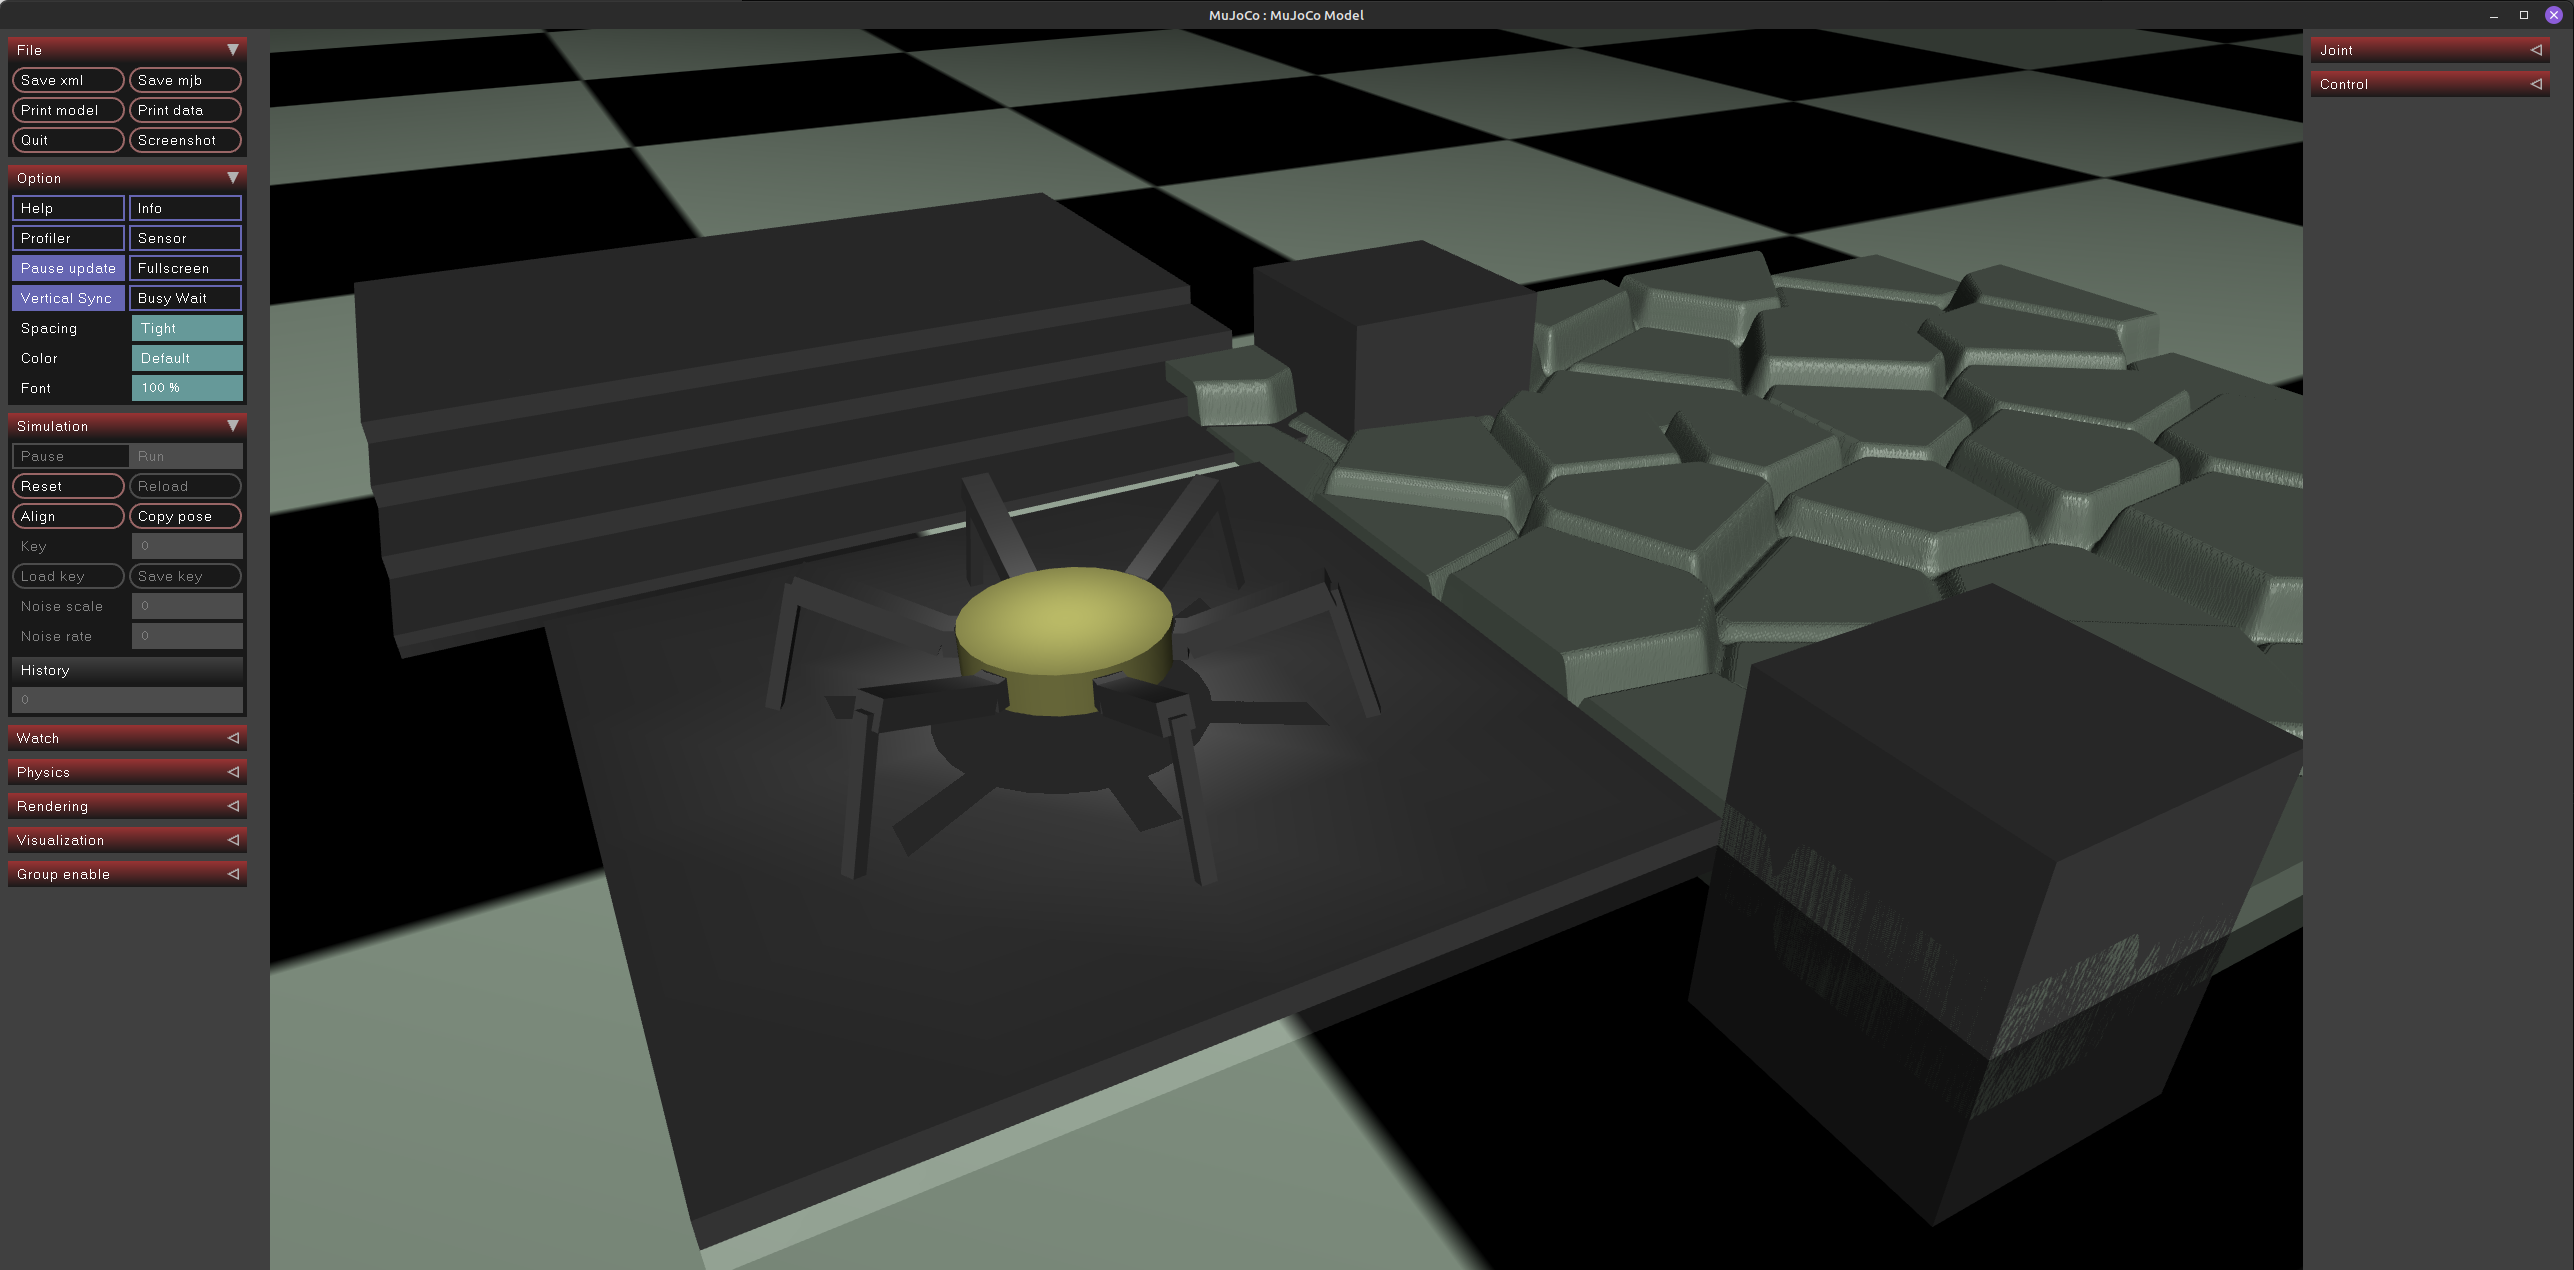
\includegraphics[height=6cm]{mujoco.png}
    \caption{The MuJoCo simulation environment}
    \label{fig:mujoco}
\end{figure}

% \bigskip
% \bigskip
% \hrule
% \smallbreak
% \hrule
